\lecture{Thu. 9/6/12}
Course information: Michael Sipser teaches the course. Alex Arkhipov and Zack Rumscrim teach the recitations. The website is 
\url{http://math.mit.edu/\~sipser/18404}.

The 3rd edition of the textbook has an extra lesson on parsing and  deterministic free languages (which we will not cover), and some additional problems. The 2nd edition is okay.

%Overpriced. ``It's a good book." Textbooks have gotten a little cuckoo. Publishing company mixture of people service to society. Less of that now.

\subsection{Overview}

\subsubsection{Computability theory}

In the first part of the course we will cover \textbf{computability theory}: what kinds of things can you solve with a computer and what kinds of things can you not solve with a computer? Computers are so powerful that you may think they can do anything. That's false. For example, consider the question

\begin{center}Does a given program meet a given specification?\end{center}

\noindent
Is it possible to build a computer that will answer this question, when you feed it any program and any specification? No; this problem is {\it uncomputable}, impossible to solve with a computer. 

Is it possible to build a computer so that when I feed it math statements (for instance, Fermat's last theorem or the twin primes conjecture), it will output true or false? Again, no. No algorithm tell whether a math statement is true or false. Not even in principle (given sufficiently long time and large space).

We'll have to introduce a formal model of computation---what do we mean by a computer?---to talk about the subject in a mathematical way. There aer several different models for computation. We'll talk about the simplest of these---finite automata---today.

Computability theory had its hayday 1930 to 1950's; it is pretty much finished as a field of research. 

\subsubsection{Complexity theory}

By contrast, the second half of the course focuses on \textbf{complexity theory}. This picks up where computability left off, from 1960's to the present. It is still a major area of research, and focuses not on whether we \emph{can} solve a problem using a computer, but how \emph{hard} is it to solve? The classical example is factoring. You can easily multiply 2 large numbers (ex. 500-digit numbers) quickly on a laptop. No one knows how or if you can do the opposite---factor a large number (ex. 1000-digit number)---easily. The state of the art is 200 digits right now. 250 digits and up is way beyond what we can do in general. %of course, if even, divide by 2.

We'll define different ways of measuring hardness: time and space (memory). We'll look at models that are specific to complexity theory, such as probabilistic models and interactive proof systems. A famous unsolved problem is the P vs. NP problem, which will be a theme throughout our lessons on complexity. In these problems, some kind of ``searching" is inevitable.

\subsubsection{Why theory?}

What is value of studying computer science theory? People question why a computer science department should invest in theoretical computer science. This used to be a big issue. 

Firstly, theory has proved its value to other parts of computer science. Many technologists and companies grew up out of the work of theorists, for example, RSA cryptography. Akamai  %formed by a colleague, coming
came out of looking at distributed systems from a theoretical point of view. %Michael's colleague.
Many key personnel in Google were theorists, because search has a theoretical side to it. Theorists have played a role in building the computer science industry.

Second, theory as a part of science. It's not just driven by its applications, but by {\it curiosity}. For example, ``how hard is factoring?" is a natural question that it is intrinsically worthwhile to answer.
Our curiosity is makes us human.

Computer science theory may also help us understand the brain in the future. We understand heart and most of our other organs pretty well, but we have only the faintest idea how the brain works. Because the brain has a computation aspect to it, it's entirely possible that some theory of computation will help solve this problem.
%A very natural theory of computation. Brain has computation aspect to it. Possibly something related. As part of our desire to understand the world. 

Is there more stuff to do? Certainly. We're still at the very beginnings of computer science and theory. Whole realms out there are worthy of exploration.

That's what and why we do this stuff.
\subsection{Finite Automata}
\subsubsection{An example}
We need to set up our models for computability theory. The first one will be finite automata. An example of a finite automata is given by the following picture.

\begin{center}
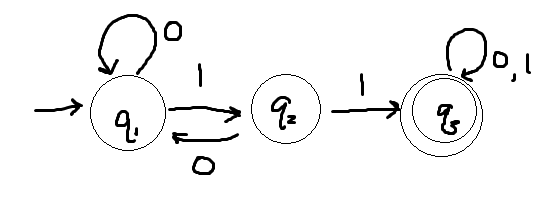
\includegraphics{1-1}
\end{center}

The \textbf{states} are $\{q_1,q_2,q_3\}$. The \textbf{transitions} are arrows with 0 or 1, such as $\xra{0}$. The \textbf{start} state is $q_1$ (it has a regular arrow leading to it) and the accept states is $\{q_3\}$ (it has a double circle). Note each state has 2 arrows exiting it, 0 and 1.

How does this automaton work when we feed it a string such as 010110? We start at the start state $q_1$. Read in the input symbols one at a time, and follow the transition arrow given by the next bit. 
\begin{itemize}
\item
0: take the arrow from $q_1$ back to $q_1$.
\item
1: take the arrow from $q_1$ to $q_2$.
\item
0: take the arrow back to $q_1$.
\item
1: get to $q_2$
\item 
1: get to $q_3$
\item 
0: stay at $q_3$.
\end{itemize}
Since $q_3$ is an accept state, the output is ``accept." By contrast, the input state 101 ends at $q_2$; the machine does not accept, i.e. it rejects the input.\\

\prbbox{
What strings does the machine accept?
}
\vskip0.15in
The machine accepts exactly the strings with two consecutive 1's. 
The language of $A$, denoted $L(A)$, is the set of accepted strings, i.e. the language that the machine recognizes.
(This term comes from linguistics.)

We say that the language of $A$ is
\[
L(A)=\set{w}{w\text{ has substring }11}.
\]

\subsection{Formalization}

We now give a formal definition of a finite automaton.
%Things can be done in formal way. At least do in this case.

\begin{df}
A \textbf{finite automaton} is a tuple $M=(Q,\Sigma,\de,q_0,F)$ where
\begin{itemize}
\item
$Q$ is a finite set of states,
\item $\Sigma$ is a finite alphabet (collection of symbols, for instance $\{0,1\}$),
\item $\de$ is the transition function that takes a state and input symbol and gives another state
\bal
\de:Q\times \Sigma&\to Q\\
(q,a)&\mapsto r.
\end{align*}
We denote this with a circle $q$ and an arrow $\xra{a}$ leading to a circle $r$.
\item
$q_0\in Q$ is a start state.
\item $F\subeq Q$ is a set of accept states.
\end{itemize}
\end{df}
To take this further, we're going to define the language of an automaton. (We did this informally by following our finger on a path. We're just doing this formally now.)
\begin{df}
Say $M$ \textbf{accepts input string} $W=W_1\cdots W_n$ where each $W_i\in \Sigma$, if $r_0,\ldots, r_n$ is a sequence from $Q$ (of states gone through) where 
\begin{itemize}
\item
$r_0=q_0$ (start at start state),
\item
$r_n\in F$ (ends at an accept state),
\item
and for each $i>0$ and each $i>0$, $r_i=\de(r_{i-1},w_i)$ (each next state is obtained the previous state by reading the next symbol and using the transition function).
\end{itemize}
The \textbf{language} of $M$ is
\[
L(M)=\set{w}{M\text{ accepts }w}.
\]
\end{df}


Note $M$ accepts certain strings and rejects certains strings, but $M$ recognizes just 1 language, the {\it collection} of all recognized strings.\footnote{If $L'$ is a subset of $L$ and $M$ recognizes $L$, we {\it don't} say $M$ recognizes $L'$.}

Note there is a special string, the empty string of length 0, denote $\ep$. By contrast, the empty {\it language} is denoted by $\phi$.

\begin{df}
A language is \textbf{regular} if some finite automaton recognizes it. 
\end{df}
For instance $\set{w}{w\text{ has substring }11}$ is a regular language because we exhibited a automaton that recognizes it.\\

\subsubsection{Building automata}

\prbbox{
Build an automaton to recognize...
\begin{itemize}
\item
The set of strings with an even number of 1's.
\item
The set of strings that start and end with the same symbol.
\end{itemize}}
\vskip0.15in
When we have a finite automaton, and we want to design an automaton for a certain task, think as follows: \\

\cpbox{The states of the automaton represent its memory. Use different states for different possibilities.
}
\vskip0.15in
For example, 
\begin{enumerate}
\item
an automaton that accepts iff the string has an even number of 1's will have to count number of 1's mod 2. You want to have one state for each possibility.
\item 
an automaton that accepts iff the first equals the last symbol will have to keep track of what the first symbol is. It should have different states for different possibilities of the first symbol.
\end{enumerate}


In the next lecutre and a half we'll seek to understand the regular languages. There are simple languages that are not regular, for example, the language that has an equal number of 0's and 1's is not regular.

\begin{proof}[Proof sketch.]
Such an automaton would have to keep track of the difference between number of 0's and 1's so far, and there are an infinite number of possibilities to track; a finite automaton has only finitely many states and can keep track of finitely many possibilities.
\end{proof}

\subsubsection{Closure properties of languages}

\begin{df}
We call the following 3 operations on languages \textbf{regular operations}.
\begin{itemize}
\item
$\cup$ union: $A\cup B=\set{w}{w\in A\text{ or }w\in B}$
\item
$\circ$ concatenation:
\[
A\circ B=AB=\set{w}{w=xy,\,x\in A,\, y\in B}.
\]
\item
$*$ Kleene star (unary operation) 
\[
A^*=\set{w}{w=X_1X_2\cdots X_k,\,k\ge 0,\,x_i\in A}.
\]
\end{itemize}
\end{df}%steven kleene's grandson, steven kleen jr. in dept! 
These are traditionally called the regular operations: they are in a sense minimal, because starting from a simple set of regular languages and applying these three operations we can get to all regular languages. %complement, intersection

\begin{ex}
If $A=\{\text{good, bad}\}$ and $B=\{\text{boy, girl}\}$ we get
\[
A\circ B=\{\text{good boy, good girl, bad boy, bad girl}\}.
\]
\end{ex}
Note for $*$, we stick together words in any way we want to get longer string. We get an infinite language unless $A\subeq\{\ep\}$. Note $\ep\in A^*$; in particular, $\phi^*=\{\ep\}$.

\begin{thm}
The collection of regular languages is closed under regular operations. In other words, if we take 2 regular languages (or 1 regular language, for ${}^*$) and apply a regular operation, we get another regular language.
\end{thm}
We say the integers are ``closed" under multiplication and addition, but not ``closed" under division, because if you divide one by another, you might not get an integer. Closed means ``you can't get out" by using the operation.
\begin{proof}[Proof of closure under $\cup$]
We show that if $A$ and $B$ are regular, then so is $A\cup B$.

We have to show how to construct the automaton for the union language given the automata that recognize $A$ and $B$, i.e. given
%The idea is to take the product set.
\bal
M_1&=\{Q_1,\Si,\de_1,q_1,F_1\}\text{ recognizing }A\\
M_2&=\{Q_2,\Si,\de_2,q_2,F_2\}\text{ recognizing }B
\end{align*}
construct $M=(Q,\Si,\de,q_0,F)$ recognizing $A\cup B$.
%build union machine.
%unpack definitions
(For simplicity, let $\Si_1=\Si_2=\Si$.)

\begin{center}
\includegraphics{1-2}
\end{center}

You might think: run the string through $M_1$, see whether $M_1$ accepts it, then run the string through $M_2$ and see whether $M_2$ accepts it. But you can't try something on the whole input string, and try another thing on the whole input string! You get only 1 pass. \\

\cpbox{Imagine yourself in the role of $M$.}
\vskip0.15in
The solution is to run both $M_1$ and $M_2$ at the same time. 
Imagine putting two fingers on the diagrams of the automata for $M_1$ and $M_2$, and moving them around. At the end, if either finger is on an accept state, then we accept. This strategy we can implement in $M$. We now formalize this idea.

We should keep track of a state in $M_1$ and a state in $M_2$ as a single state in $M$. So each state in $M$ corresponds to a pair of states, on in $M_1$ and $M_2$; let
\[Q=Q_1\times Q_2=\set{(q,r)}{q\in Q_1,\,r\in Q_2}.\]
How to define $\de$? When we get a new symbol coming in; we go to wherever $q$ goes and wherever $r$ goes, individually.
\[
\de((q,r),a)=(\de_1(q,a),\de_2(r,a)).
\]
The start state is $q_0=(q_1,q_2)$. The accept set is
\[
F=(F_1\times Q_2)\cup (Q_1\times F_2).
\]
(Note $F_1\times F_2$ gives intersection.)

It is clear by induction that the $k$th state of $M$ is just the $k$th state of $M_1$ and $k$th state of $M_2$.
\end{proof}

\prbbox{Prove that the collection of regular languages is closed under concatenation and Kleene star.}
\begin{proof}[Proof of closure under $\circ$]
To know whether a string $w$ is in $A\circ B$, we think as follows: Suppose reading from the beginning of $w$ we see a string in $A$, say $x_1\cdots x_{a_1}$. In other words, we get to an accept state in $Q_1$. Then maybe we have
\[
\underbrace{x_1\cdots x_{a_1}}_{\in A}\underbrace{x_{a_1+1}\cdots x_{n}}_{\in B}.
\]
But maybe we should keep reading until next time we get to an accept state in $Q_1$, say step $a_2$, and 
\[
\underbrace{x_1\cdots x_{a_2}}_{\in A}\underbrace{x_{a_2+1}\cdots x_{n}}_{\in B}.
\]
But maybe we have 
\[
\underbrace{x_1\cdots x_{a_3}}_{\in A}\underbrace{x_{a_3+1}\cdots x_{n}}_{\in B}!
\]
So the possibilities ``branch"---imagine putting one more finger on the diagram each time we get to an accept state; one finger then goes to $Q_2$ and the other stays at $Q_1$. Our fingers will occupy a subset of the union $A\cup B$, so let
\[
Q=2^{Q_1\cup Q_2},\text{ the set of subsets of }Q_1\cup Q_2.
\]
Now define
\[
\de(S,a)=\begin{cases}\set{\de(s,a)}{s\in S},&F_1\cap S= \phi\\
\set{\de(s,a)}{s\in S}\cup \{\de(q_2,a)\},&F_1\cap S\ne \phi.
\end{cases}
\]
The start state is $\{q_1\}$ and the accept set is
\[
F=\set{S\subeq Q}{F_2\cap S\ne \phi},
\]
i.e. the set of subsets that contain at least one element of $F_2$. Details of checking this works left to you!
\end{proof}
To be continued...